\documentclass{beamer}

\usepackage{listings}
\usepackage{framed}
\usepackage{caption}
\usepackage{color}
\usepackage{xcolor}
\usepackage{amsfonts}
\usepackage{amsmath}

\lstset{
    language=C,
    basicstyle=\ttfamily\tiny,
    frame=tb,
    %numbers=left,
    %stepnumber=1,
    %numbersep=5pt,
    backgroundcolor=\color{white},
    showspaces=false,
    showstringspaces=false,
    showtabs=false,
    tabsize=4,
    captionpos=b,
    breaklines=true,
    breakatwhitespace=true,
    keywordstyle=\color{violet},
    commentstyle=\color{magenta}\itshape,
    emphstyle=\color{cyan},
    stringstyle=\color{red},
    identifierstyle=\color{blue}
}

\usetheme{Boadilla}

\title{Introduction to C Programming}
\author{Oliver Masters \\ \texttt{oliver.masters@ibm.com}}
\date{15th August 2018}

\begin{document}

\begin{frame}
\titlepage
\end{frame}

\section{Overview of the Language}

\begin{frame}
    \frametitle{What is C?}
    \begin{itemize}[<+->]
        \item General-purpose, imperative, procedural  programming language
        \item Compiled
        \item Extremely portable
        \item Static, weak typing 
        \item Higher level than assembly, but low-level memory access available
    \end{itemize}
\end{frame}

\begin{frame}
    \frametitle{Brief history of C}
    \begin{columns}
        \column{0.5\textwidth}

        \begin{itemize}[<+->]
            \item First released 1972
            \item Bell Laboratories
            \item Developed alongside Unix by K\&R
            \item 5 standards in total, latest: C11
            \item Influenced almost every major language since
        \end{itemize}

        \column{0.25\textwidth}

        \begin{figure}
            \centering
            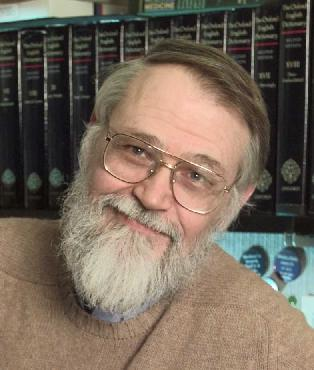
\includegraphics[width=\textwidth]{briankernighan.jpg}
            \caption*{Brian Kernighan}
            \label{fig:kern}
        \end{figure}

        \column{0.25\textwidth}

        \begin{figure}
            \centering
            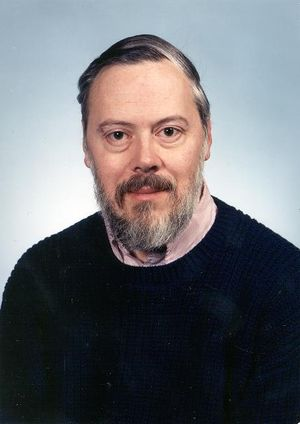
\includegraphics[scale=0.5]{dennisritchie.jpg}
            \caption*{Dennis Ritchie}
            \label{fig:ritch}
        \end{figure}
    \end{columns}
\end{frame}

\begin{frame}
    \frametitle{Why learn or use C?}
    \begin{itemize}[<+->]
        \item Extremely fast to execute
        \item Unbeatable portability
        \item Very mature -- systems critical to safety
        \item Microcontrollers/embedded systems
        \item Kernel and driver development
        \item Deeper understanding of algorithms and data structures
        \item Low-level control
    \end{itemize}
\end{frame}

\section{Technical Details}

\begin{frame}
    \frametitle{Hello World}
    \begin{figure}
        \lstinputlisting{../Code/HelloWorld/hello.c}
    \end{figure}
\end{frame}

\begin{frame}
    \frametitle{Notes on syntax}
    \begin{columns}
        \column{0.5\textwidth}
        \begin{itemize}
            \item Whitespace ignored
            \item Semicolons at ends of statements
            \item Braces
            \item Identifiers may not override keywords
        \end{itemize}
        \column{0.5\textwidth}
        \begin{table}
            \texttt{%
            \resizebox{\linewidth}{!}{%
            \begin{tabular}{| c | c | c | c |}
                \hline
                auto        & extern    & short     & while \\
                \hline
                break       & float     & signed    & \_Alignas \\
                \hline
                case        & for       & sizeof    & \_Alignof \\
                \hline
                char        & goto      & static    & \_Atomic \\
                \hline
                const       & if        & struct    & \_Bool \\
                \hline
                continue    & inline    & switch    & \_Complex \\
                \hline
                default     & int       & typedef   & \_Generic \\
                \hline
                do          & long      & union     & \_Imaginary \\
                \hline
                double      & register  & unsigned  & \_Noreturn  \\
                \hline
                else        & restrict  & void      & \_Static\_assert  \\
                \hline
                enum        & return    & volatile  & \_Thread\_local  \\
                \hline
            \end{tabular}}}
            \caption{Keywords in C11}
        \end{table}
    \end{columns}
\end{frame}

\begin{frame}
    \frametitle{Variables}
    \begin{figure}
        \lstinputlisting{../Code/Variables/variables.c}
    \end{figure}
\end{frame}

\begin{frame}
    \frametitle{Conditional execution}
    \begin{figure}
        \lstinputlisting{../Code/Conditionals/if.c}
    \end{figure}
\end{frame}

\begin{frame}
    \frametitle{While loops}
    \begin{figure}
        \lstinputlisting{../Code/While/while.c}
    \end{figure}
\end{frame}

\begin{frame}
    \frametitle{For loops}
    \begin{figure}
        \lstinputlisting{../Code/For/for.c}
    \end{figure}
\end{frame}

\begin{frame}
    \frametitle{Functions}
    \begin{figure}
        \lstinputlisting{../Code/Functions/functions.c}
    \end{figure}
\end{frame}

\begin{frame}
    \frametitle{Pointers}
    \begin{figure}
        \lstinputlisting{../Code/Pointers/pointers.c}
    \end{figure}
\end{frame}

\begin{frame}
    \frametitle{Arrays}
    \begin{figure}
        \lstinputlisting{../Code/Arrays/arrays.c}
    \end{figure}
\end{frame}

\begin{frame}
    \frametitle{Passing Arrays to Functions}
    \begin{figure}
        \lstinputlisting{../Code/PassingArrays/passingArrays.c}
    \end{figure}
\end{frame}

\begin{frame}
    \frametitle{Strings}
    \begin{figure}
        \lstinputlisting{../Code/Strings/strings.c}
    \end{figure}
\end{frame}

\begin{frame}
    \frametitle{Structs}
    \begin{figure}
        \lstinputlisting{../Code/Structs/structs.c}
    \end{figure}
\end{frame}

\begin{frame}
    \frametitle{Memory Management}
    \begin{itemize}[<+->]
        \item Can also be done dynamically
        \item No garbage collection -- \texttt{malloc} and \texttt{free}
        \item See example code in \texttt{Code/Memory/memory.c}
    \end{itemize}
\end{frame}

\begin{frame}
    \frametitle{Further reading}
    \begin{itemize}
        \item General tutorials
            \begin{itemize}
                \item \url{https://www.tutorialspoint.com/cprogramming/index.htm}
                \item \url{https://www.cprogramming.com/tutorial/c-tutorial.html}
            \end{itemize}
        \item Algorithms and data structures in C
            \begin{itemize}
                \item \url{https://www.sitesbay.com/data-structure/c-data-structure}
                \item \url{https://www.geeksforgeeks.org/data-structures/}
                \item \url{https://www.cprogramming.com/algorithms-and-data-structures.html}
            \end{itemize}
        \item Useful tools, frameworks and libraries
            \begin{itemize}
                \item \url{https://cmake.org/}
                \item \url{https://libcheck.github.io/check/}
                \item \url{http://cutest.sourceforge.net/}
                \item \url{https://www.gnu.org/software/gsl/}
                \item \url{http://www.netlib.org/lapack/}
                \item \url{https://developer.gnome.org/glib/}
                \item \url{https://curl.haxx.se/libcurl/}
                \item \url{https://www.openmp.org/}
            \end{itemize}
    \end{itemize}
\end{frame}

\begin{frame}
    \frametitle{Questions}
    \begin{itemize}
        \item Any questions?
    \end{itemize}
\end{frame}

\end{document}
